\documentclass[english]{article}
\usepackage{amsmath}
\usepackage[letterpaper]{geometry}
\usepackage[table,xcdraw]{xcolor}
\usepackage{graphicx}
\graphicspath{ {images/} }
\geometry{verbose,tmargin=1in,bmargin=1in,lmargin=1in,rmargin=1in}

\title{ESE 650 Project 3 report: Gesture recognition}
\author{Dhruva Kumar}
\date{}

\begin{document}

\maketitle

\section{Introduction}
Given the gyroscope and accelerometer readings of 6 different gestures (circle, eight, inf, etc), the task is to identify the gesture for a new sequence. 
\\ \\ Hidden Markov Models are used to learn the hidden states given the observation sequence (gyroscope and accelerometer readings) for each gesture. This is done via the EM like procedure: Baum Welch algorithm. For testing, the forward step is used to find the likelihood of the sequence given each model and the maximum is taken as the most predicted sequence. 


\section{Data preprocessing}
The raw gyroscope and accelerometer readings are used as the observation sequences/features to train the HMM model after processing it:

\begin{enumerate}
\item
The data (gyroscope and accelerometer readings) are mean centered. 
\item
The data is then smoothed using the Savitzky Golay filter. This is a FIR filter which maximizes the SNR (signal to noise ratio) based on regression. 
A low pass filter and an adaptive filter, weiner filter was tried and tested. The Savitzky Golay filter outperformed these two. It smoothed out the signals better and maintained the periodicity among the repeating sequences. The weiner filter did not work so well since because of its adaptive nature, the periodicity among the repeating sequences was lost. This periodicity is important to learn the states for the particular gesture. 
\item
On observation of the data, it was found to contain static parts in the starting and end. Since this does not contribute to the states, it was removed. The trimming was done by finding when the slope of the signal crossed a certain threshold and that was marked as the start point. The same was done for the end point. 
\end{enumerate}

\paragraph{Quantization of observation}
After cleaning up the data, the sequences were discretized using kmeans clustering. 20 clusters were chosen to split the data into. The six dimensional centroids were retained to quantize new test sequences. The norm of the new test sequence and every centroid was computed and the minimum taken to find the cluster which the new sequence closely belongs to.

\section{Initial model parameters}
After cross validation, the following initial parameters were chosen for the final model:
\\\\ Number of states (N): 10
\\ Number of clusters (M): 20
\\ HMM structure: Left to right with the last node connected to the first one and self loops.
\\ $\pi$: [1,0,0...N] - begins with the first state.
\\ $A$: band diagonal (based on the structure) of random values
\\ $B$: random values
\\\\
\begin{figure}[h]
\centering
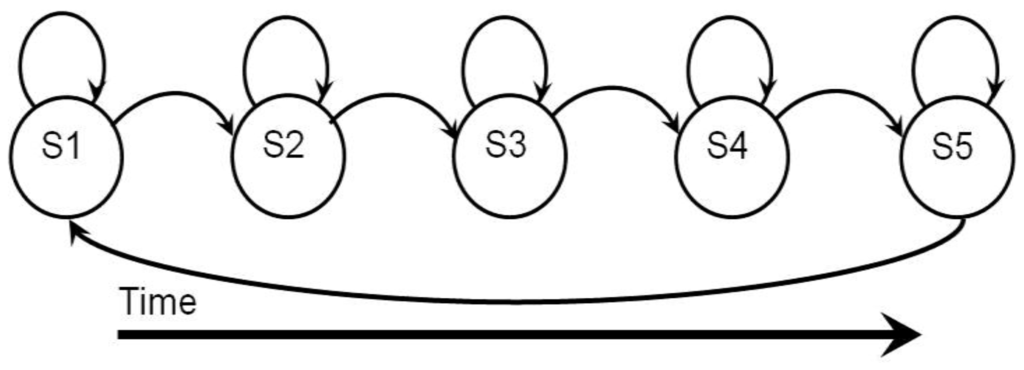
\includegraphics[scale = 2]{struct}
\caption{HMM left to right structure used}
\end{figure}

A left to right model worked slightly better than a fully connected one for different values of $N$ and $M$. After convergence of the learning procedure, it was found that the transition matrix $A$ of the fully connected structure more or less resulted in a diagonal matrix, implying an inherent left to right structure in the model. A left to right model converged faster and sometimes gave better results. 

\paragraph{Vectorization:}
To speed up the process of cross validation over different parameters, the code was substantially vectorized, specifically at the forward, backward and the update of $A$ and $B$ steps. 
%\\\\Tested on the Baum Welch procedure for 5 sequences and 1 iteration :
\begin{table}[h]
\centering
\caption{Effect of vectorization for 5 sequences and 1 iteration}
\begin{tabular}{|l|l|}
\hline
\textbf{Vectorization} & \textbf{Time taken (seconds)} \\ \hline
Unvectorized code & \textbf{4.514} \\ \hline
Vectorized & \textbf{0.86} \\ \hline
\end{tabular}
\end{table}
%\\Unvectorized code:  \textbf{4.514 seconds}
%\\Vectorized code: \textbf{0.86 seconds}


\section{Learning: Baum Welch}
The HMM model was learnt using the Baum Welch procedure. It is an iterative EM procedure alternating between the E and M step, trying to maximize the cost function $P(O|\lambda)$ until a convergence criteria is met. 
\\\\ \textbf{Initialization:}
\\The initial model \{$\pi$, $A$, $B$\} is taken as described in the section above.
\\\\ \textbf{Expectation:} 
Given model, compute the forward and backward variables $\alpha$ and $\beta$
\\This comprises of the forward and backward step. It computes $P(O|\lambda)$, the probability of the likelihood of the observation sequence, given the model by computing the forward $\alpha$ and backward $\beta$ variables. 
\\The scaling as described in the Rabiner paper \cite{c1} is used.
\begin{itemize}
\item Forward procedure (compute $\alpha$):

\begin{enumerate}
	\item Initialization:
	\begin{align*}
	\alpha_1(i) =&\; \pi_i b_i(O_1) & 1 \leq i \leq N \\
	c_1 =&\; \frac{1}{\sum_{i=1}^N \alpha_1(i)} \\
	\hat{\alpha_1}(i) =&\; c_1 \alpha_1(i)  
	\end{align*}

	\item Induction:
	\begin{align*}
	\alpha_{t+1}(j) =&\; [ \sum_{i=1}^N \alpha_t(i) a_{ij} ] \ b_j(O_{t+1}) & 1 \leq t \leq T-1, \ \leq j \leq N \\
	c_t =&\; \frac{1}{\sum_{i=1}^N \alpha_t(i)} \\
	\hat{\alpha_t}(t) =&\; c_t \alpha_t(i)  
	\end{align*}

	\item Termination:
	\begin{align*}
	P(O|\lambda) =&\; \sum_{i=1}^N \alpha_T(i) \\
	=&\; \frac{1}{\prod_{\tau=1}^T c_{\tau}} \\ 
	=&\; \frac{1}{C_T} \\ 
	\log{P(O|\lambda)} =&\;  -\sum_{t=1}^T \log{c_t}\\
	\end{align*}
\end{enumerate}

\item Backward procedure (compute $\beta$):
\\(Using the same scaling computed from $\alpha$)
\begin{enumerate}
	\item Initialization:
	\begin{align*}
	\beta_T(i) =&\; 1  & 1 \leq i \leq N \\
	\hat{\beta_T}(i) =&\; c_T \beta_T(i)
	\end{align*}

	\item Induction:
	\begin{align*}
	\beta_T(i) =& \sum_{j=1}^N a_{ij} b_j(O_{t+1}) \beta_{t+1}(j) & T-1 \geq t \geq 1, \ 1 \leq i \leq N \\
	\hat{\beta_t}(i) =&\; c_t \beta_t(i)	
	\end{align*}

\end{enumerate}
\end{itemize} 
For multiple sequences, $\alpha^l$, $\beta^l$ and $c^l$ for each sequence $l$ is computed.  \\ \\
\textbf{Modification:} 
Given $\alpha$ and $\beta$, compute most likely model \{$\pi$, $A$, $B$\}.
\\ We adjust \{$\pi$, $A$, $B$\} to maximize the cost function: $P(O|\lambda)$. The re-estimated paramters {$\bar{\pi}$, $\bar{A}$, $\bar{B}$} are as follows:
\begin{align*}
	\bar{\pi_i} =&\; \text{expected number of times in state } S_i \text{ at time } (t = 1)  \\
	=&\; \gamma_1(i) \\
	\bar{a}_{ij} =&\; \frac{\text{expected number of transitions from state }S_i \text{ to } S_j}{\text{expected number of transitions from state }S_i} \\
	=&\; \frac{\sum_{t=1}^{T-1} \xi_t(i,j)}{\sum_{t=1}^{T=1}\gamma_t(i)} \\
	=&\; \frac{\sum_{t=1}^{T-1} \alpha_t(i) a_{ij} b_{j}(O_{t+1}) \beta_{t+1}(j)}{\sum_{t=1}^{T-1} \alpha_t(i) \beta_{t}(j) } \\
	=&\; \frac{\sum_{t=1}^{T-1} \hat{\alpha}_t(i) a_{ij} b_{j}(O_{t+1}) \hat{\beta}_{t+1}(j)}{\sum_{t=1}^{T-1} \hat{\alpha}_t(i) \hat{\beta}_{t}(j) / c_t } \\
	\text{For multiple observations, }\\
	=&\; \frac{\sum_{l=1}^{L-1} \sum_{t=1}^{T_l-1} \hat{\alpha}_t^{l}(i) a_{ij} b_{j}(O_{t+1}^{l}) \hat{\beta}_{t+1}^{l}(j)}{\sum_{t=1}^{T_l-1} \hat{\alpha}_t^{l}(i) \hat{\beta}_{t}^{l}(j) / c_t^{l} }\\ \\
\end{align*}

\begin{align*}
	\bar{b}_j(k) =&\; \frac{\text{expected number of times in state } j \text{ and observing symbol }\upsilon_k}{\text{expected number of times in state }j} \\
	=&\; \frac{\sum_{t=1, O_t=\upsilon_k}^{T} \gamma_t(j)}{\sum_{t=1}^{T} \gamma_t(j)} \\
	=&\; \frac{\sum_{t=1, O_t=\upsilon_k}^{T} \hat{\alpha}_t(j) \hat{\beta}_t(j) / c_t}{\sum_{t=1}^{T} \hat{\alpha}_t(j) \hat{\beta}_t(j) / c_t} \\
	\text{For multiple observations, } \\
	=&\;  \frac{\sum_{l=1}^{L} \sum_{t=1, O_t^{l}=\upsilon_k}^{T_l} \hat{\alpha}_t^{l}(j) \hat{\beta}_t^{l}(j) / c_t^{l}}{\sum_{t=1}^{T_l} \hat{\alpha}_t^{l}(j) \hat{\beta}_t^{l}(j) / c_t^{l}} \\
\end{align*}

$\gamma_t(i)$ is the probability of being in state i at time t given the observations sequence and the model $\lambda$
\begin{align*}
	\gamma_t(i) =&\; P(q_t = S_i | O, \lambda) = \frac{\alpha_t(i) \beta_t(i)}{P(O | \lambda)} \\ 
\end{align*}

$\xi_t(i,j)$ is the probability of being in state $S_i$ at time $t$ and $S_j$ at time $t+1$, given the model and observation sequence. 
\begin{align*}
	\xi_t(i,j) =&\; P(q_t = S_i, q_{t+1} = S_j | O,\lambda) = \frac{\alpha_t(i) a_{ij} b_j(O_{t+1}) \beta_{t+1}(j)}{P(O|\lambda)} \\
\end{align*}

\textbf{Convergence criteria}: The convergence criteria was assigned as when the absolute of the difference in the log likelihood of $P(O|\lambda)$ between successive iterations is less than 0.1 \\

\begin{figure}[h]
\centering
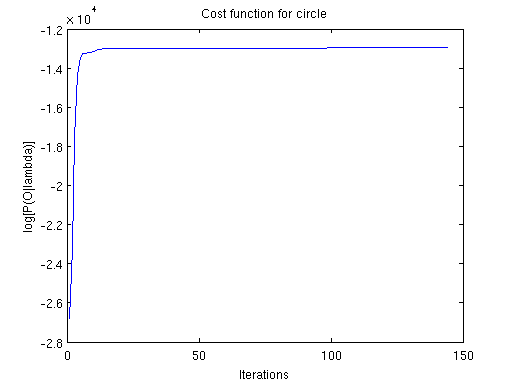
\includegraphics[scale=0.6]{cost}
\caption{Cost function for circle after running Baum Welch}
\end{figure}


\section{Testing and results}
Once the models were generated for each gesture, testing on the test sequences was done using the forward procedure. The forward procedure gives us $P(O|\lambda)$, i.e. the likelihood of the test sequence, given the models. The maximum value among the models was chosen as the most likely gesture. \\

\begin{table}[h]
\centering
\caption{Confusion matrix for the in sample training data is given below}
\label{my-label1}
\begin{tabular}{lcccccc}
       & beat3                     & beat4                     & circle                    & eight                     & inf                       & wave                      \\
beat3  & \cellcolor[HTML]{FFFFC7}4 & 1                         & 0                         & 0                         & 0                         & 0                         \\
beat4  & 1                         & \cellcolor[HTML]{FFFFC7}4 & 0                         & 0                         & 0                         & 0                         \\
circle & 0                         & 0                         & \cellcolor[HTML]{FFFFC7}5 & 0                         & 0                         & 0                         \\
eight  & 0                         & 0                         & 0                         & \cellcolor[HTML]{FFFFC7}5 & 0                         & 0                         \\
inf    & 0                         & 0                         & 0                         & 1                         & \cellcolor[HTML]{FFFFC7}4 & 0                         \\
wave   & 0                         & 0                         & 0                         & 0                         & 0                         & \cellcolor[HTML]{FFFFC7}5
\end{tabular}
\end{table}


The accuracy on the \textbf{sample test} set given = \textbf{100\%} \\ 

Cross validation was done by setting aside 10 random sequences from 30 sequences of the training data as test sequences. The rest were used for training.  \\

\begin{table}[h]
\centering
\caption{Cross validation accuracy for different parameters}
\begin{tabular}{|c|c|c|}
\hline
\textbf{N} & \textbf{M} & \textbf{CV accuracy} \\ \hline
10 & 20 & 80\% \\ \hline
15 & 20 & 70\% \\ \hline
15 & 15 & 70\% \\ \hline
25 & 20 & 80\% \\ \hline
35 & 20 & 60\% \\ \hline
45 & 20 & 60\% \\ \hline
50 & 20 & 70\% \\ \hline
70 & 20 & 60\% \\ \hline
\end{tabular}
\end{table} 

\begin{table}[h]
\centering
\caption{Cross validation accuracy with N=10, M=20 for different structures}
\label{my-label}
\begin{tabular}{|c|c|}
\hline
\textbf{HMM structure} & \textbf{CV accuracy} \\ \hline
\begin{tabular}[c]{@{}c@{}}Left to right with self loops and\\ last node connected to the first one\end{tabular} & 80\% \\ \hline
Fully connected & 80\% \\ \hline
\end{tabular}
\end{table}

The HMM structure did not make much of a difference. The fully connected model reduced somewhat to a left-right model after learning. The left-right model was much faster and therefore used. 


%\bibliographystyle{unsrt}%Used BibTeX style is unsrt
%\bibliography{sample}

\begin{thebibliography}{99}
\bibitem{c1} Lawrence R. Rabiner, ‘A Tutorial on Hidden Markov Models and Selected Applications
in Speech Recognition,’ Proceedings of the IEEE, Vol. 77, No. 2, pp.257-286, February, 1989
\bibitem{c3} http://courses.media.mit.edu/2010fall/mas622j/ProblemSets/ps4/tutorial.pdf
\end{thebibliography}

\end{document}
